\documentclass[a4paper,9pt]{extarticle}
\usepackage[dutch]{babel}
% Package to make citations superscrit with brackets
\usepackage[super,square]{natbib}
\RequirePackage{times}
\usepackage[scaled]{inconsolata}
\usepackage{graphicx} 
\usepackage{titlesec}
\usepackage{amsmath}
\usepackage[hypcap=true]{caption}  % of report, book, etc.
\titleformat{\section}
  {\normalfont\LARGE\bfseries}
  {\thesection}{1em}{}  



% Package to change margin size
\usepackage{anysize}
\marginsize{1.5cm}{1.5cm}{1cm}{1cm}

\usepackage{lastpage}

\usepackage{listings}
% Package to make headers


\usepackage{xcolor}
% Kleuren gebaseerd op je screenshot
\definecolor{codepurple}{RGB}{153, 0, 102}     
\definecolor{codeorange}{RGB}{0, 0, 0}         
\definecolor{codeblue}{RGB}{0, 0, 0}           
\definecolor{codegreen}{RGB}{0, 128, 0}        
\definecolor{codegray}{RGB}{0, 0, 0}  
\definecolor{codedarkblue}{RGB}{0, 0, 139}        % 

 % iets grijzer achtergrond
\definecolor{background}{RGB}{255, 255, 255}  
% donkergrijze tekst
\lstset{
  language=Python,
  backgroundcolor=\color{background},
  basicstyle=\ttfamily\small\color{codegray},
  numbers=left,
  numberstyle=\tiny\color{gray},
  numbersep=7pt,
  frame=single,
  framesep=2pt,
  rulecolor=\color{codegray},
  keywordstyle=\color{codepurple},
  stringstyle=\color{codeorange},
  identifierstyle=\color{codeblue},
  commentstyle=\color{codegreen},
  moredelim=[s][\color{codegreen}]{"""}{"""},
  showstringspaces=false,
  aboveskip=1em,
  belowskip=1em,
  breaklines=true,
  breakatwhitespace=true,
  emph={build_feedforward_model},
  emphstyle=\color{codedarkblue},
}
\usepackage{fancyhdr}
\renewcommand{\headrulewidth}{0pt}
\cfoot{}
% Package for highligths
\usepackage{soul}
% Colors for the references links
\usepackage[dvipsnames]{xcolor}
% Package to link references
\usepackage{hyperref}
\hypersetup{
    colorlinks=true,
    linkcolor=black,
    citecolor=CadetBlue,
    filecolor=CadetBlue,      
    urlcolor=CadetBlue,
}
% Package for lorem ipsum
%\usepackage{lipsum}
% Package for multicolumn
\usepackage{multicol}
% Package for removing paragraph identations
\usepackage{parskip}
\setlength\columnsep{18pt}
% Sets bastract
\renewenvironment{abstract}
 {\par\noindent\textbf{Samenvatting}\ \ignorespaces \\}
 {\par\noindent\medskip}

\begin{document}
% Makes header
\pagestyle{fancy}
\fancyhead[R]{\textit{PEE51}}
\fancyhead[C]{\textit{Elektrotechniek}}
\fancyhead[L]{\textit{Hogeschool Rotterdam}}
\fancyfoot[L]{M. Reints \& T. van Ommeren}
\fancyfoot[C]{}
\fancyfoot[R]{pagina \thepage\ van \pageref{LastPage}}
% Makes footnotes with an asterisk
\renewcommand*{\thefootnote}{\fnsymbol{footnote}}
\begin{center}
  \huge{\textbf{Is het mogelijk om een PID controller te vervangen door een AI?}} \\
  \vspace{0.2cm}

\vspace{0.2cm}
\normalsize
Mitchel Reints - \href{mailto:1040953@hr.nl}{1040953@hr.nl} \\
Thomas van Ommeren - \href{mailto:1033239@hr.nl}{1033239@hr.nl} \\
\vspace{0.1cm}
\textit{Hogeschool Rotterdam - Elektrotechniek - PEE51} 
\vspace{0.1cm} \\
\today
\medskip
\normalsize
\end{center}
\begin{abstract}
In dit onderzoek wordt onderzocht of een neuraal netwerk het gedrag van een PID-regelaar kan nabootsen of verbeteren in een systeem waarbij een pingpongbal op een ingestelde hoogte wordt gehouden. De huidige regeling werkt met een PID-regelaar, maar het afstellen hiervan is tijdrovend en gevoelig voor omgevingsfactoren. Door een machine learning-model te trainen met data van het systeem, wordt onderzocht of een alternatief regelalgoritme mogelijk is. Er wordt niet ingegaan op de implementatie van het netwerk in een embedded omgeving, maar er wordt wel rekening gehouden met de beperkingen van de NXP FRDM-MCXN947 microcontroller, waarop het model uiteindelijk moet draaien. Het onderzoek richt zich op de technische haalbaarheid en de prestatievergelijking tussen het neurale netwerk en de traditionele PID-regelaar.
\end{abstract}
{\color{gray}\hrule}
\begin{multicols}{2}
\setlength{\headheight}{14.49998pt}
\titleformat{\section}
  {\normalfont\LARGE\bfseries\centering}
  {\thesection}{1em}{}  
%\tableofcontents

\section{Inleiding}
Hogeschool Rotterdam beschikt over de cursus Digitale Systemen (DIS10) over een opstelling waarbij een pingpongbal op een ingestelde hoogte wordt gehouden. Deze opstelling bestaat uit een verticale buis met onderaan een ventilator. Door de luchtdruk van de ventilator wordt de bal omhoog geblazen. Met behulp van een microcontroller wordt de ventilator aangestuurd, zodat de bal op een gewenste hoogte blijft zweven. De regeling van de ventilatorsnelheid gebeurt momenteel met behulp van een PID-regelaar (Proportioneel-Integrerend-Differentieel), waarbij de afwijking tussen de gewenste en werkelijke hoogte continu wordt bijgestuurd.

Hoewel deze opstelling functioneert zoals bedoeld, is het instellen van de PID-parameters vaak een handmatig proces. Het vergt tijd om het systeem goed af te stemmen om het uiteindelijk stabiel te laten reageren op hoogteveranderingen. Daarnaast kunnen veranderingen in de omgeving (zoals temperatuur of luchtvochtigheid) de prestaties van de PID-regelaar beïnvloeden.

De begeleidende docent heeft de vraag gesteld of deze traditionele regelmethode vervangen kan worden door een benadering gebaseerd op machine learning. Machine learning biedt de mogelijkheid om op basis van data te leren hoe het systeem zich moet gedragen. In dit project wordt onderzocht of het mogelijk is om een machine learning model te ontwikkelen dat het gedrag van de PID-regelaar kan nabootsen of zelfs verbeteren.

Dit onderzoek is relevant omdat het laat zien hoe klassieke regeltechniek vervangen kan worden door moderne, zelflerende systeem. Daarnaast sluit het aan bij actuele ontwikkelingen binnen de techniek en biedt het studenten inzicht in zowel embedded systemen als kunstmatige intelligentie. Uiteindelijk is het doel om een demonstratie-opstelling te creëren die gebruikt kan worden tijdens bijvoorbeeld open dagen, om zo op een toegankelijke manier beide technieken te tonen.

Het doel van dit onderzoek is om te onderzoeken of een neuraal netwerk het gedrag van een PID-regelaar effectief kan nabootsen of verbeteren in een systeem waarbij een pingpongbal op een ingestelde hoogte wordt gehouden. Hierbij wordt een model ontwikkeld, getraind en geëvalueerd in een gesimuleerde omgeving. Uiteindelijk moet het model geschikt zijn voor implementatie op een embedded platform, met als doel een stabiele en nauwkeurige hoogtecontrole te realiseren. Het onderzoek richt zich op zowel de technische haalbaarheid als de vergelijking met de bestaande PID-regelaar.

Voor dit onderzoek zijn er een aantal onderzoeksvragen geformuleerd die uiteindelijk de hoofdvraag van dit onderszoek moeten beantwoorden:
\begin{enumerate}
  \item Hoe werkt een PID-regelaar en hoe wordt deze toegepast in de huidige opstelling?
  \item Welke soorten neurale netwerken zijn geschikt voor regeltoepassingen in embedded systemen?
  \item Hoe kan trainingsdata verzameld worden om het gedrag van de PID-regelaar na te bootsen?
  \item Hoe presteert het getrainde neurale netwerk vergeleken met de traditionele PID-regelaar?
  \item Wat zijn de beperkingen van het gebruik van een neuraal netwerk in een embedded omgeving?
\end{enumerate}

aan het einden van het onderzoek zullen deze deelvragen worden beantwoord en onderbouwd, zodat de hoofdvraag kan worden beantwoord: \textit{Is het mogelijk om een PID-regelaar te vervangen door een AI?}

Voor dit onderzoek wordt gewerkt met de **NXP FRDM-MCXN947 Development board** als microcontrollerplatform. Hoewel de oorspronkelijke DIS10-opstelling gebaseerd is op de **Texas Instruments SimpleLink Wi-Fi CC3230S Development kit**, is er door de opdrachtgever gekozen het onderzoek uit te voeren op een ander platform. Dit verschil in hardware heeft geen invloed op dit onderzoek, omdat de PID ook geintergreerd kan worden op de NXP FRDM-MCXN947 Development board.


In dit rapport wordt eerst de benodigde theorie besproken (hoofdstuk 2), gevolgd door de gebruikte methoden (hoofdstuk 3) waarin we dit onderzoek doen. Daarna worden de resultaten gepresenteerd (hoofdstuk 4) en besproken (hoofdstuk 5). Het rapport sluit af met conclusies (Hoofdstuk 6) en aanbevelingen (hoofdstuk 7).

Een neuraal netwerk\footnote{Een \textit{neuraal netwerk} is een model geïnspireerd op het menselijk brein.} wordt getraind met data.


\setlength{\headheight}{14.49998pt}
\titleformat{\section}
  {\normalfont\huge\bfseries\centering}
  {\thesection}{1em}{}  

\vspace{0.2cm}
{\color{gray}\hrule}
  



\section{Theorie}


\subsection{Werking van een PID-regelaar}

Een PID-regelaar (Proportioneel-Integrerend-Differentiërend)\cite{WikipediaPID2024}\cite{Franklin1995_PID} is een veelgebruikte terugkoppelingsregelaar in de regeltechniek, die als doel heeft een systeem naar een gewenste waarde (setpoint) te sturen door continu het verschil (de fout) tussen die gewenste waarde en de gemeten systeemoutput te corrigeren.
De PID-regelaar bestaat uit drie componenten:
\begin{itemize}
  \item \textbf{Proportioneel (P):} Deze component reageert op de huidige fout. Hoe groter de fout, hoe sterker de aansturing. Dit zorgt voor een directe correctie, maar kan leiden tot een blijvende fout (steady-state error) als deze component alleen wordt gebruikt.
  \item \textbf{Integrerend (I):} Deze component reageert op de opgetelde (geïntegreerde) fout in de tijd. Hierdoor kan de regelaar kleine resterende fouten wegwerken en wordt het systeem naar het exacte setpoint geduwd. Te veel integratie kan echter leiden tot traagheid of instabiliteit.
  \item \textbf{Differentiërend (D):} Deze component reageert op de snelheid waarmee de fout verandert. Dit helpt om snelle veranderingen te dempen en voorkomt overshoot door het systeem te vertragen voordat het het setpoint bereikt. De D-term maakt het systeem reactiever en stabieler bij plotselinge veranderingen.
\end{itemize}
De regeloutput \( u(t) \) van een PID-regelaar wordt meestal als volgt beschreven:
\begin{equation}
u(t) = K_p \cdot e(t) + K_i \cdot \int_0^t e(\tau)\,d\tau + K_d \cdot \frac{de(t)}{dt}
\label{eq:pid}
\end{equation}
waarbij:
\[
\begin{aligned}
e(t) &= r(t) - y(t) \quad \text{(de fout tussen de referentie en gemeten waarde)} \\
K_p  &= \text{proportionele versterkingsfactor} \\
K_i  &= \text{integrerende versterkingsfactor} \\
K_d  &= \text{differentiërende versterkingsfactor}
\end{aligned}
\]
Een goed afgestemde PID-regelaar zorgt voor een snelle respons, minimale overshoot en een stabiele benadering van het setpoint zonder blijvende fout. Hoewel we in dit onderzoek niet in detail ingaan op de afstemming van PID-parameters, is het belangrijk te vermelden dat dit een cruciaal onderdeel is van het gebruik van PID-regelaars in de praktijk. De afstemming wordt meestal handmatig gedaan en dit is meestal een iteratief proces waarbij de waarden van \(K_p\), \(K_i\) en \(K_d\) worden aangepast op basis van de prestaties van het systeem. Er zijn verschillende methoden voor PID-afstemming, zoals de Ziegler-Nichols-methode, maar deze vallen buiten de scope van dit onderzoek. In dit onderzoek richten we ons op het vervangen van de PID-regelaar door een neuraal netwerk, waarbij we de nadruk leggen op het gedrag van de PID regelaar en de mogelijkheid om dit gedrag te repliceren met een neuraal netwerk.
\subsection{Neurale netwerken - basisprincipes}
\cite{GeeksRNN2024}\cite{Vijayvargia2018}Een neuraal netwerk is een wiskundig model dat is geïnspireerd op de werking van het menselijk brein. Het bestaat uit een verzameling onderling verbonden knopen, ook wel neuronen genoemd, die georganiseerd zijn in lagen: één inputlaag, één of meerdere verborgen lagen en één outputlaag. Elke verbinding tussen neuronen heeft een gewicht dat bepaalt hoe sterk een input wordt doorgegeven. Tijdens het doorlopen van het netwerk wordt elke input vermenigvuldigd met het bijbehorende gewicht, opgeteld met een bias en vervolgens door een activatiefunctie gehaald. Deze activatiefunctie bepaalt of en in welke mate het neuron wordt geactiveerd. Het leerproces van een neuraal netwerk gebeurt aan de hand van trainingsdata. Op basis van de fout tussen de voorspelde output en de werkelijke waarde worden de gewichten aangepast met behulp van een algoritme zoals bijvoorbeeld backpropagation in combinatie met gradient descent. Door herhaaldelijk trainen op veel voorbeelden leert het netwerk patronen en relaties herkennen in de data. Neurale netwerken zijn bijzonder krachtig in het modelleren van complexe, niet-lineaire systemen, en worden daarom veel gebruikt in toepassingen zoals beeldherkenning, spraakherkenning en regeltechniek.
\begin{center}
\centering
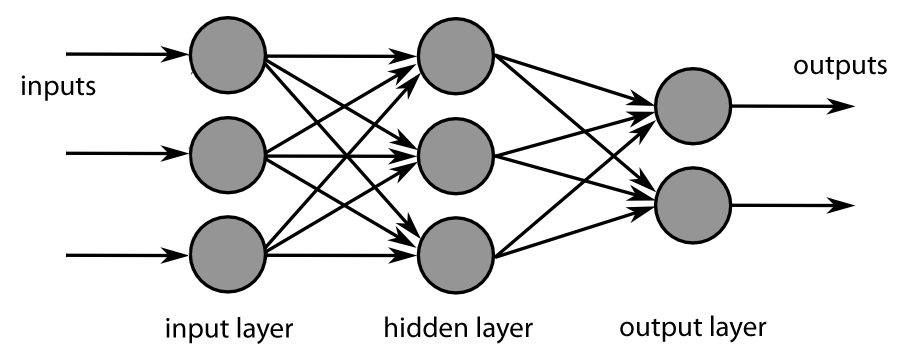
\includegraphics[width=0.45\textwidth]{./afbeeldingen/Neuraalnetwerkpng.png}
\label{fig:Illustratie_neuraal_netwerk}
\captionof{figure}{Illustratie van een neuraal netwerk}
\end{center}
\subsection{vergelijking PID versus NN-regelaars}
Zowel PID-regelaars als neurale netwerken kunnen worden ingezet om systemen te regelen, maar hun werking, toepassingsgebied en eigenschappen verschillen sterk.
\subsubsection{Verschillen}
\begin{itemize}
  \item \textbf{Regelprincipe:} Een PID-regelaar is gebaseerd op een vaste wiskundige formule die werkt met de fout tussen gewenste en gemeten waarden. Een neuraal netwerk leert juist op basis van voorbeelddata een model van het systeemgedrag.
  \item \textbf{Aanpasbaarheid:} PID-regelaars hebben vaste parameters \(K_p\), \(K_i\), \(K_d\) die handmatig of via tuning bepaald worden. Neurale netwerken leren automatisch complexe relaties tijdens het trainen, zonder expliciet geprogrammeerde regels. 
  \item \textbf{Complexiteit:} PID-regelaars zijn relatief eenvoudig te implementeren en begrijpen. Neurale netwerken zijn complexer en vereisen meer rekenkracht en data.
  \item \textbf{Flexibiliteit:} PID is minder geschikt voor sterk niet-lineaire systemen of systemen met veel vertraging. Neurale netwerken kunnen deze situaties beter aan, mits voldoende training.
  \item \textbf{Transparantie:} PID-regelaars zijn goed uitlegbaar. Neurale netwerken zijn vaak 'black boxes', waarbij het moeilijk is om te achterhalen waarom een bepaalde beslissing wordt genomen.
\end{itemize}
\subsubsection{Overeenkomsten}
\begin{itemize}
  \item Beide regelmethoden kunnen gebruikt worden voor het aansturen van dynamische systemen.
  \item Beide maken gebruik van foutsignalen (in neurale netwerken impliciet tijdens het trainen).
  \item Beide kunnen met feedback werken om de systeemoutput te corrigeren.
  \item Beide vereisen afstemming of training om goed te presteren in een specifieke toepassing.
\end{itemize}







\subsection{keuze van netwerkarchitecturen }


Voordat er in gegaan wordt op de NN-architecturen voor deze toepassing is het belangrijk om met een aantal factoren rekening mee te houden. Deze factoren zijn van belang bij het kiezen van een geschikte NN-architectuur voor het vervangen van een PID-regelaar in een embedded systeem. De factoren die onderandere worden besproken zijn:
\begin{itemize}
  \item \textbf{Real-time vereisten:} Als het systeem real-time reacties vereist, moet de gekozen architectuur snel genoeg zijn om aan deze eisen te voldoen. Dit kan de keuze beperken tot lichtere netwerken of optimalisaties zoals quantisatie.
  \item \textbf{Ondersteuning voor embedded systemen:} De gekozen architectuur moet compatibel zijn met de hardware van het embedded systeem, zoals microcontrollers of FPGA's. Dit kan beperkingen opleggen aan de complexiteit en het type netwerk.
  \item \textbf{Ondersteuning voor machine learning frameworks:} Het is belangrijk om te kiezen voor machine learning frameworks die ondersteuning bieden voor embedded systemen, zoals TensorFlow Lite, Keras of PyTorch Mobile. Deze frameworks zijn ontworpen om neurale netwerken te optimaliseren en te implementeren op beperkte hardware.
  \item \textbf{Trainings- en implementatietijd:} De tijd die nodig is om het neuraal netwerk te trainen en te implementeren, kan ook een factor zijn bij de keuze van de architectuur. Sommige netwerken vereisen meer tijd voor training en afstemming dan andere.
\end{itemize}


Aan de hand van deze factoren kunnen we een weloverwogen keuze maken voor de netwerkarchitectuur die het beste past bij de specifieke toepassing en de vereisten van het systeem. Het is belangrijk om de juiste balans te vinden tussen complexiteit, prestaties en implementatiegemak, zodat het neuraal netwerk effectief kan functioneren als vervanging voor de PID-regelaar. Hieronder worden enkele architecturen die overwogen kunnen worden voor het vervangen van een PID-regelaar door een neuraal netwerk met hun voor- en nadelen:
\begin{itemize}  
  \item \textbf{Recurrente netwerken\cite{Haykin2009_recurrent} (RNN):} Deze netwerken zijn ontworpen om tijdsafhankelijke data te verwerken door informatie van eerdere tijdstappen te onthouden. Ze zijn nuttig voor systemen waarbij de huidige output afhankelijk is van eerdere inputs, zoals bij dynamische systemen. RNN's kunnen echter complexer zijn om te trainen en vereisen meer rekenkracht.
  \item \textbf{Convolutioneel Neuraal Netwerk\cite{Haykin2009_convolutional} (1D CNN):} Een 1D CNN is specifiek geschikt voor sequentiële of tijdsgebaseerde data, zoals signalen (bijvoorbeeld audio of ECG), tijdreeksen (zoals beursdata of temperatuurmetingen) en reeksen met meerdere features (zoals sensorwaarden). Hoewel convolutionele netwerken vooral bekend zijn uit de beeldverwerking, kunnen 1D CNN's effectief patronen en lokale afhankelijkheden in tijdreeksen herkennen, waardoor ze ook toepasbaar zijn voor regeltoepassingen waarbij de input bestaat uit opeenvolgende meetwaarden.
  \item \textbf{Long Short-Term Memory (LSTM):} Dit is een type RNN dat speciaal is ontworpen om lange-termijn afhankelijkheden te onthouden. LSTM's zijn zeer geschikt voor systemen met complexe dynamiek en tijdsafhankelijke gedragspatronen, maar ze zijn ook complexer en vereisen meer data om goed te presteren.
\end{itemize}

Voor de toepassing van het vervnagen van een PID-regelaar zijn er aantal kenmerken die belangrijk zijn bij het kiezen van een geschikte netwerkarchitectuur:
\begin{itemize}
  \item \textbf{Eenvoudige structuur:} Voor een microcontroller is het belangrijk dat de netwerkarchitectuur eenvoudig genoeg is om efficiënt te trainen en te implementeren. Complexe netwerken zoals LSTM's kunnen te veel rekenkracht vereisen en zijn moeilijker te optimaliseren voor embedded systemen.
  \item \textbf{Compact model:} Het model moet klein genoeg zijn om op de microcontroller te passen, wat betekent dat het aantal parameters beperkt moet zijn. Dit kan worden bereikt door het aantal lagen en neuronen te beperken, of door technieken zoals quantisatie toe te passen.
  \item \textbf{Snelle inferentie:} De gekozen architectuur moet snel genoeg zijn om real-time voorspellingen te doen, wat betekent dat de inferentietijd laag moet zijn. Dit kan worden bereikt door gebruik te maken van efficiënte activatiefuncties en optimalisaties in de netwerkstructuur.
  \item \textbf{Robuustheid:} Het netwerk moet robuust zijn tegen verstoringen en veranderingen in de systeemparameters. Dit kan worden bereikt door het netwerk te trainen op een breed scala aan scenario's en variaties in de data.
  \item \textbf{Ondersteuning voor embedded systemen:} De gekozen architectuur moet compatibel zijn met de hardware van het embedded systeem, zoals microcontrollers of FPGA's. Dit kan beperkingen opleggen aan de complexiteit en het type netwerk.
  \item \textbf{Ondersteuning voor machine learning frameworks:} Het is belangrijk om te kiezen voor machine learning frameworks die ondersteuning bieden voor embedded systemen, zoals TensorFlow Lite, Keras of PyTorch Mobile. Deze frameworks zijn ontworpen om neurale netwerken te optimaliseren en te implementeren op beperkte hardware.
  \item \textbf{Flexibiliteit in tijdsvenster:} De architectuur moet in staat zijn om te werken met verschillende tijdsvensters van inputdata, zodat het netwerk kan worden aangepast aan de specifieke toepassing en de vereisten van het systeem.
\end{itemize}
Deze kenmerken helpen bij het selecteren van een netwerkarchitectuur die geschikt is voor het vervangen van een PID-regelaar in een embedded systeem. Het is belangrijk om de juiste balans te vinden tussen complexiteit, prestaties en implementatiegemak, zodat het neuraal netwerk effectief kan functioneren als vervanging voor de PID-regelaar.


uiteindelijk is er gekozen voor een Convolutioneel Neuraal Netwerk (1D CNN) als de meest geschikte architectuur voor het vervangen van een PID-regelaar in een embedded systeem. Deze keuze is gebaseerd op de volgende overwegingen:
\begin{itemize}
  \item \textbf{Eenvoudige structuur:} Een 1D CNN heeft een overzichtelijke en relatief eenvoudige architectuur, waardoor het netwerk efficiënt te trainen en te implementeren is, zeker in vergelijking met complexere netwerken zoals LSTM's.
  \item \textbf{Compact model:} 1D CNN's kunnen worden geoptimaliseerd tot compacte modellen met een beperkt aantal parameters, wat ze geschikt maakt voor embedded systemen met beperkte rekenkracht en geheugen.
  \item \textbf{Snelle inferentie:} Door hun efficiënte structuur bieden 1D CNN's doorgaans snellere inferentie dan recurrente netwerken, wat essentieel is voor real-time toepassingen.
  \item \textbf{Robuustheid en generalisatie:} 1D CNN's zijn effectief in het herkennen van patronen en lokale afhankelijkheden in sequentiële data, waardoor ze goed kunnen generaliseren naar verschillende scenario's en bestand zijn tegen verstoringen.
  \item \textbf{Geschikt voor embedded systemen:} Er zijn diverse machine learning frameworks, zoals TensorFlow Lite en Keras, die 1D CNN's ondersteunen en optimaliseren voor gebruik op embedded hardware.
  \item \textbf{Brede frameworkondersteuning:} 1D CNN's worden breed ondersteund door populaire machine learning frameworks, wat de ontwikkeling, optimalisatie en implementatie vereenvoudigt.
  \item \textbf{Flexibiliteit in tijdsvenster:} Met 1D CNN's kan eenvoudig worden bepaald over welk tijdsvenster inputdata wordt geanalyseerd, waardoor het netwerk flexibel inzetbaar is voor uiteenlopende regeltoepassingen.
\end{itemize}
Deze overwegingen maken de 1D CNN een geschikte keuze voor het vervangen van een PID-regelaar in een embedded systeem. Het biedt een goede balans tussen prestaties, eenvoud en implementatiegemak, waardoor het effectief kan functioneren als vervanging voor de PID-regelaar in verschillende toepassingen.








\subsection{Vergelijking van prestaties}
De prestaties van een neuraal netwerk in vergelijking met een PID-regelaar kunnen op verschillende manieren worden beoordeeld, afhankelijk van de specifieke toepassing en de doelstellingen van de regeling. Enkele belangrijke prestatie-indicatoren zijn:
\begin{itemize}
  \item \textbf{Nauwkeurigheid:} Hoe goed het neuraal netwerk de gewenste output kan voorspellen in vergelijking met de PID-regelaar. Dit kan worden gemeten aan de hand van de fout tussen de voorspelde en werkelijke waarden.
  \item \textbf{Stabiliteit:} Hoe stabiel het systeem is bij het bereiken van de gewenste output. Een PID-regelaar kan soms oscillaties vertonen, terwijl een goed getraind neuraal netwerk deze kan verminderen of elimineren.
  \item \textbf{Snelheid:} Hoe snel het neuraal netwerk kan reageren op veranderingen in de input. Dit is vooral belangrijk in real-time toepassingen waar snelle aanpassingen nodig zijn.
  \item \textbf{Robuustheid:} Hoe goed het neuraal netwerk presteert onder verschillende omstandigheden, zoals verstoringen of veranderingen in de systeemparameters. Een PID-regelaar kan soms gevoelig zijn voor veranderingen in de omgeving, terwijl een neuraal netwerk mogelijk beter kan generaliseren.
\end{itemize}
De vergelijking van prestaties tussen een neuraal netwerk en een PID-regelaar kan worden uitgevoerd door beide systemen te testen op dezelfde set van inputs en de resultaten te vergelijken. Dit kan bijvoorbeeld worden gedaan door simulaties uit te voeren of door het systeem in de praktijk te testen. Het is belangrijk om de prestaties onder verschillende omstandigheden te evalueren, zoals bij verstoringen of veranderingen in de systeemparameters, om een goed beeld te krijgen van de effectiviteit van het neuraal netwerk in vergelijking met de PID-regelaar.




\subsection{Implementatie op embedded systemen}
Een van de uitdagingen van het implementeren van een neuraal netwerk is de integratie ervan in embedded systemen. Embedded systemen zijn vaak beperkt in termen van rekenkracht, geheugen en energieverbruik, wat betekent dat de implementatie van een neuraal netwerk op deze systemen specifieke overwegingen vereist. Daarom is het belangrijk om de volgende aspecten in overweging te nemen bij de implementatie van een neuraal netwerk op embedded systemen:
\begin{itemize}
  \item \textbf{Modeloptimalisatie:} Het neuraal netwerk moet worden geoptimaliseerd voor de beperkte rekenkracht en geheugen van het embedded systeem. Dit kan onder meer het verminderen van het aantal parameters, het gebruik van quantisatie of het toepassen van modelcompressie omvatten.
  \item \textbf{Efficiënte inferentie:} De inferentie (voorspellingsfase) van het neuraal netwerk moet efficiënt worden uitgevoerd. Dit kan worden bereikt door gebruik te maken van speciale hardwareversnellers, zoals Tensor Processing Units (TPU's) of Field Programmable Gate Arrays (FPGA's), die zijn ontworpen voor het uitvoeren van neurale netwerken.
  \item \textbf{Real-time prestaties:} Het neuraal netwerk moet in staat zijn om real-time voorspellingen te doen, wat betekent dat de inferentietijd snel genoeg moet zijn om te voldoen aan de vereisten van de toepassing. Dit kan worden bereikt door het netwerk te optimaliseren voor snelheid en door gebruik te maken van efficiënte algoritmen.
  \item \textbf{Compatibiliteit met hardware:} Het neuraal netwerk moet compatibel zijn met de specifieke hardware van het embedded systeem. Dit kan onder meer het gebruik van specifieke bibliotheken of frameworks omvatten die zijn geoptimaliseerd voor de gekozen hardware.
  \item \textbf{Ondersteuning voor machine learning frameworks:} Het is belangrijk om te kiezen voor machine learning frameworks die ondersteuning bieden voor embedded systemen, zoals TensorFlow Lite, Keras of PyTorch Mobile. Deze frameworks zijn ontworpen om neurale netwerken te optimaliseren en te implementeren op beperkte hardware.
\end{itemize}
 
Deze microcontroller is geschikt voor embedded toepassingen en biedt voldoende mogelijkheden voor het uitvoeren van machine learning taken. Hieronder volgt een uitgebreid overzicht van de belangrijkste kenmerken van de NXP FRDM-MCXN947\cite{NXP2025_datasheet} Development board, gebaseerd op de officiële NXP-pagina:
\begin{itemize}
  \item \textbf{Processor:} De FRDM-MCXN947\cite{NXP2025_datasheet} is uitgerust met een dual-core ARM Cortex-M33 processor, draaiend op maximaal 150~MHz per core. Deze cores zijn ontworpen voor deterministische prestaties en ondersteunen TrustZone-technologie voor beveiligde toepassingen. De gecombineerde rekenkracht (~750 DMIPS per core) maakt deze geschikt voor besturingslogica, preprocessing en embedded AI-taken.
  \item \textbf{Neural Processing Unit (NPU):} De geïntegreerde eIQ Neutron NPU biedt tot 16 GOPS (Giga Operations Per Second) rekenkracht voor machine learning-inferentie. De NPU versnelt modellen met tientallen keren vergeleken met CPU-only uitvoering. Bijvoorbeeld: een keyword spotting-model van 30~kB haalt inferentietijden van enkele milliseconden met een nauwkeurigheid van 97.06\%.
  \item \textbf{Geheugen:} De MCU bevat 2~MB on-chip flash in dual-bank configuratie, geschikt voor firmware updates tijdens runtime. Daarnaast is er 512~kB SRAM beschikbaar. Voor grotere modellen of datasets kan via SPI een externe micro-SD-kaart worden toegevoegd.
  \item \textbf{Machine learning frameworks:} TensorFlow Lite for Microcontrollers en het NXP eIQ framework worden ondersteund. Deze frameworks maken optimalisatie via quantisatie, pruning en compressie mogelijk, essentieel voor inferentie op embedded hardware.
  \item \textbf{Real-time prestaties:} Dankzij een systeemtimer, nested vectored interrupt controller (NVIC), DMA-ondersteuning en hardwarematige versnelling van AI-taken kan het systeem realtime inferenties uitvoeren (bijvoorbeeld 1--5 ms per inferentie bij kleine modellen).
\end{itemize}
Deze kenmerken maken de NXP FRDM-MCXN947 Development board een geschikte keuze voor het implementeren van een neuraal netwerk als vervanging voor een PID-regelaar in embedded systemen. Door rekening te houden met de mogelijkheden en beperkingen van deze microcontroller, kan het neuraal netwerk worden geoptimaliseerd voor de specifieke toepassing en de vereisten van het systeem.



\setlength{\headheight}{14.49998pt}
\titleformat{\section}
  {\normalfont\huge\bfseries\centering}
  {\thesection}{1em}{}  

\vspace{0.2cm}
{\color{gray}\hrule}
% 3. Methode (nog niet in pdf aanwezig)

% Doel: Beschrijf hoe jullie het onderzoek uitgevoerd hebben.

% Moet bevatten:
% 	•	Hoe is data verzameld (bijv. via simulatie of loggen van PID-gedrag)?
% 	•	Hoe is het neuraal netwerk opgezet, getraind en gevalideerd?
% 	•	Welke tools/software zijn gebruikt?
% 	•	Beschrijving van de testopstelling of simulatieomgeving.

\section{Methode}

In dit hoofdstuk wordt beschreven op welke manier het onderzoek is uitgevoerd. De focus ligt op de software-omgeving, de manier van dataverzameling, de opbouw en training van het neuraal netwerk, en de testomgeving waarin het model is geëvalueerd.

\subsection{Software en tools}

Voor zowel de simulatie van de pingpongbal-opstelling als het opzetten en trainen van het neuraal netwerk is gebruik gemaakt van Python. De volgende libraries en tools zijn ingezet:
\begin{itemize}
    \item \textbf{NumPy} en \textbf{Pandas}: voor het verwerken en analyseren van data;
    \item \textbf{Matplotlib} voor visualisatie van resultaten;
    \item \textbf{TensorFlow} en \textbf{Keras}: voor het bouwen, trainen en valideren van het neuraal netwerk;
    \item \textbf{Scikit-learn}: voor data preprocessing en evaluatiemethoden;
    \item \textbf{Jupyter Notebook}: voor het ontwikkelen en testen van de code in iteraties.
\end{itemize}

\subsection{Dataverzameling}

De trainingsdata voor het neuraal netwerk is verzameld door een simulatie van de bestaande PID-regelaar. In deze simulatie werd het gedrag van de PID-regelaar gelogd terwijl deze een pingpongbal op verschillende hoogtes stabiel probeerde te houden. Hierbij zijn gegevens zoals tijd, doelhoogte, werkelijke hoogte, fout, fout intergratie, fout afgeleide en bijbehorende PWM-waarden opgeslagen.

De data werd vervolgens gesplitst in een trainingsset (80\%) en een validatieset (20\%).

\subsection{Neuraal netwerk opzetting}

Op basis van de kenmerken van het systeem en de vereisten voor embedded implementatie is gekozen voor een 1D Convolutioneel Neuraal Netwerk (1D CNN). Dit type netwerk is efficiënt in het herkennen van patronen in sequentiële data en heeft relatief lage rekenvereisten.

De architectuur van het netwerk bestaat uit:
\begin{itemize}
    \item Een inputlaag met vensters van opeenvolgende foutwaarden;
    \item Een of meerdere 1D convolutionele lagen met ReLU-activatie;
    \item Een flatten-laag gevolgd door één dense laag;
    \item Een outputlaag die de benodigde PWM-waarde voorspelt.
\end{itemize}

\subsection{Trainingsstrategie en hyperparameters tuning}
Het model is getraind met behulp van backpropagation en de Adam optimizer. De volgende hyperparameters zijn getest en afgestemd:
\begin{itemize}
    \item Learning rate: $0.001$, $0.0005$, $0.0001$;
    \item Batch size: 32 en 64;
    \item Aantal epochs: 50–200;
    \item Rechthoekige activatievensters: lengte 5–20 samples.
\end{itemize}

De performance van het model werd tijdens de training geëvalueerd met behulp van de mean squared error (MSE). Early stopping werd toegepast om overfitting te voorkomen.

\subsection{Testopstelling of Simulatieomgeving}

De opstelling is volledig gesimuleerd in Python, waarbij de dynamiek van de pingpongbal in een verticale buis werd gemodelleerd. Hierbij werd rekening gehouden met de krachten op de bal (zwaartekracht, luchtdruk door de ventilator) en de vertraging in het systeem. Zowel de PID-regelaar als het neuraal netwerk werd getest in dezelfde simulatieomgeving zodat een eerlijke vergelijking kon worden gemaakt.

Het gedrag van beide regelstrategieën werd geëvalueerd op responsietijd, stabiliteit, overshoot, en robuustheid bij verstoringen.









\vspace{0.2cm}
{\color{gray}\hrule}
\section{Resultaten}
% 4. Resultaten (nog niet in pdf aanwezig)

% Doel: Laat zien wat het neurale netwerk presteerde t.o.v. PID.

% Moet bevatten:
% 	•	Grafieken of tabellen die prestaties tonen.
% 	•	Vergelijking met PID-regelaar (gebruik prestatiecriteria uit 2.5).
% 	•	Eventueel foutenanalyse of validatie.


\subsection{Resultaten van de getrainde modellen}

\subsection{vergelijking met de PID-regelaar}

\subsection{Effect van variatie in data/robuustheid}

\subsection{Observatie tijdens simulatie}




\vspace{0.2cm}
{\color{gray}\hrule}
\section{Discussie}
% 5. Discussie (nog niet in pdf aanwezig)

% Doel: Reflecteer op de resultaten.

% Moet bevatten:
% 	•	Interpretatie: waarom presteerde het NN beter/slechter?
% 	•	Wat zijn de sterke/zwakke punten van jullie aanpak?
% 	•	Wat zou je in vervolgonderzoek anders doen?
% 	•	Zijn de beperkingen van het embedded platform realistisch meegenomen?



\subsection{Interpetatie van de resultaten}

\subsection{Beperkingen van het model}

\subsection{Lessen en inzichten}

\subsection{Reflectie op de aanpak}



\setlength{\headheight}{14.49998pt}
\titleformat{\section}
  {\normalfont\huge\bfseries\centering}
  {\thesection}{1em}{}  

\vspace{0.2cm}
{\color{gray}\hrule}
\section{Conclusie en Aanbevelingen}
% 6. Conclusie en aanbevelingen (nog niet in pdf aanwezig)

% Doel: Beantwoord de hoofdvraag en geef advies.

% Moet bevatten:
% 	•	Kort antwoord op de hoofdvraag.
% 	•	Samenvatting van belangrijkste bevindingen.
% 	•	Aanbevelingen voor praktijk of toekomstig onderzoek.
% 	•	Eventueel suggesties voor daadwerkelijke implementatie.



\subsection{Beantwoording van de hoofdvraag}

\subsection{Samenvatting van de belangrijke bevindingen}

\subsection{Aanbevelingen voor implementatie}

\subsection{Suggesties voor vervolgonderzoek}




\bibliographystyle{plain}
\bibliography{references}
%\section*{Begrippenlijst}
\begin{description}
  \item[PID-regelaar] Een regelsysteem dat gebruikmaakt van proportionele, integrale en afgeleide termen.
  \item[Neuraal netwerk] Een algoritme geïnspireerd op het menselijk brein dat patronen leert herkennen.
  \item[Backpropagation] Methode om foutmarges in een neuraal netwerk terug te voeren en gewichten aan te passen.
\end{description}
\end{multicols}

\titleformat{\section}
  {\normalfont\LARGE\bfseries}
  {\thesection}{1em}{} 
%\appendix
\section{Meetresultaten}
\label{appendix:meetresultaten}

In deze bijlage worden de meetresultaten weergegeven die zijn verzameld tijdens de experimenten.

\section{Tabel met resultaten}
Hieronder staat een overzichtstabel van de gemeten waarden.

\begin{table}[h!]
\centering
\begin{tabular}{|c|c|c|}
\hline
Tijd (s) & Spanning (V) & Stroom (A) \\
\hline
0.0 & 3.30 & 0.10 \\
1.0 & 3.28 & 0.11 \\
2.0 & 3.27 & 0.12 \\
\hline
\end{tabular}
\caption{Gemeten waarden tijdens test 1}
\end{table}

\section{Grafiek}
Hier zie je een voorbeeld van een grafiek (je moet je eigen figuur invoegen):

\begin{figure}[h!]
\centering
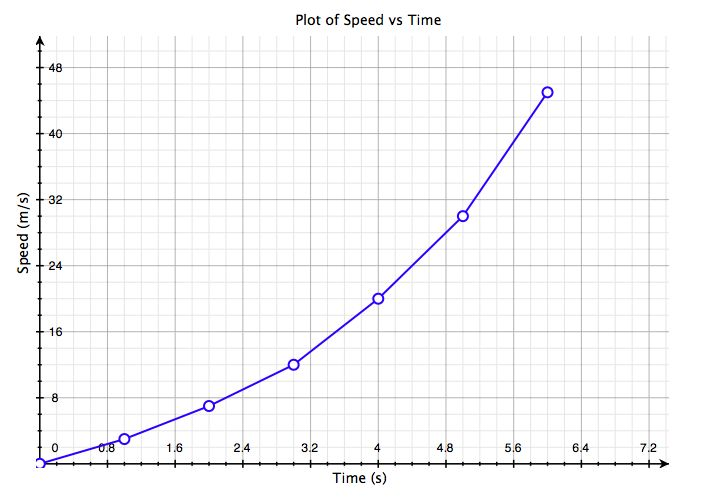
\includegraphics[width=0.7\textwidth]{./afbeeldingen/grafiek.jpeg}
\caption{Spanning over tijd}
\label{fig:spanning_tijd}
\end{figure}

\section{Broncode}
\label{appendix:broncode}

\section{python-script}
\begin{lstlisting}[language=Python, numbers=left, breaklines=true, basicstyle=\ttfamily\scriptsize]
    def build_feedforward_model(input_layer_size, hidden_layer_size, output_layer_size):
        """Bouw een neuraal netwerkmodel volgens TensorFlow-conventies."""
        model = keras.Sequential(name="Feedfoward_Model")
        model.add(layers.Input(shape=(input_layer_size,), name="Input_Layer"))
        model.add(layers.Dense(hidden_layer_size, activation='sigmoid', name="Hidden_Layer"))
        model.add(layers.Dense(hidden_layer_size_2, activation='sigmoid', name="Hidden_Layer_2"))
        model.add(layers.Dense(output_layer_size, activation='softmax', name="Output_Layer"))
        return model 
\end{lstlisting}
 
\end{document}